We will now consider a complementary approach to the path integral, based around the Fokker-Planck equation.
This is a different formalism for stochastic processes, in contrast to the Langevin-equation approach taken in the previous chapter.
We derive the Fokker-Planck equation from the Kramers–Moyal expansion.

\section{Kramers-Moyal expansion}

To derive the Kramers-Moyal expansion, consider a particle with a certain initial condition, so $\Pe(x, t = 0) = \delta(x)$.
Then its probability distribution for later times \emph{equals} the conditional probability that it started at that point.
That is, $\Pe(x, t) = \Pe(x, t| x = 0, t=0)$.
We will only consider continuous Markov processes.
The Chapman-Kolgomorov equation, \autoref{eq: chapman kolgomorov cont}, for a time-step $\Delta t$ is then
%
\begin{align}\label{eq: CK for KM}
    \Pe(x, t + \Delta t) = \int \dd x' \Pe(x, t + \Delta t) \Pe(x', t).
\end{align}
%
We now define the \emph{conditional moments},
%
\begin{align}
    K^{(n)}(x', t, \Delta t)
    =
    \E{\left[ x(t + \Delta t) - x(t) \right]^n}_{x(t) = x'}
    =
    \int \dd x \, (x - x')^n \Pe(x, t + \Delta t|x', t).
\end{align}
%
The subscript on the expectation value here indicates the initial conditions $x'$ at $t$.
To derive the KM-expansion, we rewrite the delta-function as
%
\begin{align}
    \delta(x - y)
    = \delta(x' - x + y - x')
    & =
    \sum_{n = 0}^\infty
    \frac{1}{n!} (y - x')^n
    \left( \pdv{  }{ x' } \right)^n \delta(x' - x)\\
    & =
    \sum_{n = 0}^\infty
    \frac{(-1)^n}{n!} (y - x')^n
    \left( \pdv{  }{ x } \right)^n \delta(x' - x).
\end{align}
%
Here, we have Taylor-expanded the delta function, and change the variable with respect to which we differentiate in the last line.
The derivative of the dirac-delta function is defined if we consider it in terms of an integral together with a test-function $f(x)$---we then integrate by parts, so
%
\begin{align}
    \int \dd x\, \delta'(x - x_0) f(x) = - \int \dd x\, \delta(x-x_0) f'(x) = - f'(x_0),
\end{align}
%
and so on.

Inserting this into the trivial rewriting, 
%
\begin{align}
    \Pe(x, t + \Delta t| x', t) = \int \dd y\, \delta(y - x) \Pe(y, t + \Delta t | x', t).
\end{align}
%
we get
%
\begin{align}
    \Pe(x, t + \Delta t | x', t)
    & =
    \sum_{n = 0}^\infty
    \frac{(-1)^n}{n!} 
    \left( \pdv{  }{ x } \right)^n \delta(x' - x)
    \int \dd y \, (y - x')^n \Pe(y, t + \Delta t| x', t)\\
    & =
    \delta(x' - x) + 
    \sum_{n = 1}^\infty
    \frac{(-1)^n}{n!} 
    \left( \pdv{  }{ x } \right)^n \left[\delta(x' - x) K^{(n)}(x', t, \Delta t)\right].
\end{align}
%
Combining this rewriting with the Chapman-Kolgomorov, \autoref{eq: CK for KM}, and expanding in $\Delta t$, we get
%
\begin{align}
    \Pe(x, t + \Delta t) - \Pe(x, t) & = \Delta t \pdv{ \Pe(x, t) }{ t } + \Oh(\Delta t^2) \\
    & = \int \dd x' \Pe(x, t + \Delta t|x', t) \Pe(x', t) - \Pe(x, t) \\
    & = 
    \int \dd x' \,
    \left\{
        \delta(x' - x) + 
        \sum_{n = 1}^\infty
        \frac{(-1)^n}{n!} 
        \left( \pdv{  }{ x } \right)^n \left[\delta(x' - x) K^{(n)}(x, t, \Delta t)\right]
    \right\}
    \Pe(x', t)
    - \Pe(x, t)\\
    & = 
    \sum_{n = 1}^\infty
    \frac{(-1)^n}{n!} 
    \left( \pdv{  }{ x } \right)^n \left[\Pe(x, t) K^{(n)}(x, t, \Delta t)\right] 
\end{align}
%
\todo{This is maybe a bit fast with integral by parts and everyting...}
We define the \emph{Kramers-Moyal coefficients},
%
\begin{align}
    \D^{(n)}(x, t) \equiv \lim_{\Delta t \rightarrow 0 } \frac{K^{(n)}(x, t, \Delta t)}{n! \Delta t},
\end{align}
%
which means that we can, in the limit $\Delta t\rightarrow 0$, write
%
\begin{align}
    \pdv{ \Pe(x, t) }{ t }
    =
    \sum_{n = 1}^\infty
    (-1)^n
    \left( \pdv{  }{ x } \right)^n \left[\Pe(x, t) \D^{(n)}(x, t)\right] .
\end{align}
%
This is the Kramers-Moyal equation.

We thus have an invitation series which gives the time-evolution of the Kramers-Moyal coefficients, which depend on the conditional moments.
However, in many cases this simplifies.
In fact, there are only three cases, as given by \emph{Pawula's theorem}.
The cases are

(1) The series is truncated at $n = 1$, so $\D^{(n)} = 0$ for $n > 1$.
This corresponds to deterministic evolution of $\Pe(x, t) = \delta(x - x(t))$, and the Kramers-Moyal equation becomes Liouville's equation.

(2) The series is truncated at $n = 2$. This gives the Fokker-Planck equation, and will be what we concern ourselves with.

(3) The sarees is infinite, and any truncation leads to non-positive probability densities.
It is usually this in this case the equation is called the ``Kramers-Moyal equation''.

\begin{framed}
    \noindent
    \textit{Proof of Pawula's theorem:}
    We sketch the proof of the theorem here.
    It is based on (as so many proofs) Schwartz inequality,
    %
    \begin{align}
        \left[
            \int \dd x\, p(x) f(x) g(x)
        \right]^2
        \leq
        \int \dd x\, p(x) f^2(x)
        \int \dd x\, p(x) g^2(x).
    \end{align}
    %
    In this case, $p(x) = \Pe(x', t, + \Delta t | x, t)$, and
    %
    \begin{align}
        f(x) & = 
        \begin{cases}
            (x - x')^{\frac{ m - 1 }{ 2 }}, & \text{if } m \text{ is odd and } m\geq 3\\
            (x - x')^{\frac{ m - 2 }{ 2 }}, & \text{if } m \text{ is even and } m\geq 4
        \end{cases},\\
        g(x) & = 
        \begin{cases}
            (x - x')^{\frac{ m + 1 }{ 2 }}, & \text{if } m \text{ is odd and } m\geq 3\\
            (x - x')^{\frac{ m + 2 }{ 2 }}, & \text{if } m \text{ is even and } m\geq 4
        \end{cases}.
    \end{align}
    %
    Then, the inequality becomes between conditional moments.
    On the left-hand side, switching $x'\rightarrow x$\textcolor{red}{IS THIS RIGHT?}
    %
    \begin{align}
        \left[
            \int \dd x\, p(x) f(x) g(x)
        \right]^2
        = \left[K^m(x, t, \Delta t)\right]^2
    \end{align}
    %
    Consider $m$ even, then the right-hand side is
    %
    \begin{align}
        \int \dd x\, p(x) f^2(x)
        \int \dd x\, p(x) g^2(x)
        =
        K^{m-1}(x, t, \Delta t)
        K^{m+1}(x, t, \Delta t),
    \end{align}
    %
    so, applying with $ \lim_{\Delta t\rightarrow 0} \frac{ 1 }{ \Delta t^{2m} }$, the inequality becomes
    %
    \begin{align}
        \D^{m}(x, t) &\leq \frac{ (m-1)! (m+1)! }{ (m!)^2 } \D^{m-1}(x, t) \D^{m+1}(x, t),
        &&
        m \text{ odd and } m \geq 3.
    \end{align}
    %
    In the case of $m$ even, we instead get
    %
    \begin{align}
        \D^{m}(x, t) &\leq \frac{ (m-2)! (m+2)! }{ (m!)^2 } \D^{m-2}(x, t) \D^{m+2}(x, t),
        &&
        m \text{ even and } m \geq 4.
    \end{align}
    %
    We see now that the different coefficients are linked together in an infinite chain.
    We leave it as an exercise to show that if $\D_r = 0$ for any $r \geq 3$, then $\D_m = 0$ for all $m \geq 0$.
\end{framed}

\section{Connection to the Langevin equation}

Consider the Langevin equation in the Itô discretization,
%
\begin{align}
    \odv{  }{ t } x(t)
    \overset{\alpha=0}{=}
    a_I(x(t), t) + b_I(x(t), t) \eta(t).
\end{align}
%
Then, the Kramers-Moyal coefficients are
%
\begin{align}
    D^{(1)}(x, t) & = a_I(x, t), &
    D^{(2)}(x, t) & = \frac{ 1 }{ 2 } b_I^2(x, t), &
    D^{(n)}(x, t) & = 0, \quad n > 2.
\end{align}
%
\begin{framed}
    \noindent
    \textit{Exercise:} Derive the Kramers-Moyal coefficients given above.
\end{framed}
We therefore get case (3) of Pawula's theorem, and the Kramers-Moyal equation reduces to the Fokker-Plank, which takes the form
%
\begin{align}
    \partial_t \Pe(x, t)
    = - \partial_x \left[a_I(x, t) \Pe(x, t)\right] + \frac{ 1 }{ 2 } \partial_x^2 \left[b_I(x, t)^2 \Pe(x, t)\right].
\end{align}
%
On the other hand, if we instead consider an equation with the Stratonovich discretization,
%
\begin{align}
    \odv{  }{ t } x(t)
    \overset{\alpha=\frac{1}{2}}{=}
    a_S(x(t), t) + b_S(x(t), t) \eta(t),
\end{align}
%
we have the following relationship, from the change-of-discrization formula \autoref{eq: change of discrtization},
%
\begin{align}
    a_I(x, t) &= a_S(x, t) + \frac{ 1 }{ 2 } b_S(x, t) \partial_x b_S(x, t), \\
    b_I(x, t) & = b_I(x, t).
\end{align}
%
Therefore, the corresponding Fokker-Planck is
%
\begin{align}
    \partial_t \Pe(x, t)
    & = - \partial_x \left[\left\{a_S(x, t) + \frac{ 1 }{ 2 } b_S(x, t) \partial_x b_S(x, t) \right\} \Pe(x, t)\right] 
    + \frac{ 1 }{ 2 } \partial_x^2 \left[b_S(x, t)^2 \Pe(x, t)\right] \\
    & = - \partial_x \left[a_S(x, t)  \Pe(x, t)\right] 
    + \frac{ 1 }{ 2 } \partial_x \left\{ b_S(x, t)\partial_x \left[ b_S(x, t) \Pe(x, t)\right] \right\}.
\end{align}
%
In higher dimensions, the Langevin equations, where $\bm x\in \R^n$ and $\bm \eta \in \R^m$,
%
\begin{align}
    \odv{  }{ t } x_i
    &\overset{\alpha=0}{=}
    - \partial_i a_{I,i}(\bm x, t) + B_{I,ij}(\bm x, t) \eta_j(t),\\
    \odv{  }{ t } x_i
    &\overset{\alpha=\frac{1}{2}}{=}
    - \partial_i a_{S,i}(\bm x, t) + B_{S,ij}(\bm x, t) \eta_j(t),\\
\end{align}
%
correspond to the following Fokker-Plancks:
%
\begin{align}
    \partial_t \Pe(\bm x, t) 
    & = - \partial_i \left[A_{I,i}(\bm x, t) \Pe(\bm x, t)\right]
    + \frac{ 1 }{ 2 } \partial_i \partial_j \left[B_{I, ik}(\bm x, t) B_{I, j k}(\bm x, t) \Pe(\bm x, t)\right], \\
    \partial_t \Pe(\bm x, t) 
    & = - \partial_i \left[A_{S,i}(\bm x, t) \Pe(\bm x, t)\right]
    + \frac{ 1 }{ 2 } \partial_i \left\{ B_{S, ik}(\bm x, t) \partial_j  \left[ B_{S, j k}(\bm x, t) \Pe(\bm x, t)\right] \right\},
\end{align}
%
where we have used Einstein's summation convention.


\subsection*{Underdamped equation}

If consider have an underdamped equation for a particle,
%
\begin{align}
    \odv{  }{ t } \bm x & = \bm v, \\
    m \odv{  }{ t } \bm v &= - \gamma \bm v - \bm \nabla U(\bm x) + \sqrt{ 2 \gamma k_B T } \bm \eta(t),
\end{align}
%
where
%
\begin{align}
    \E{\eta_i(t) \eta_j(t')} = \delta_{ij} \delta(t),
\end{align}
%
then the corresponding Fokker-Planck equation is called \emph{Kramers equation}, and models the probability distribution of both velocity and position.

\subsection*{Overdamped equation}

In the limit $m/\gamma\rightarrow 0$, the above equation becomes an over-damped equation,
%
\begin{align}
    \odv{  }{ t } \bm x &=  - \mu\bm \nabla U(\bm x) + \sqrt{ 2 \mu k_B T } \bm \eta(t),
\end{align}
%
where $\mu = 1 / \gamma$ is the mobility.
The corresponding Fokker-Planck is
%
\begin{align}
    \partial_t \Pe(\bm x, t)
    =
    \mu \bm \nabla \cdot \left[ \left(\bm \nabla U(\bm x) + \mu k_B T \bm \nabla\right) \Pe(\bm x, t)\right].
\end{align}
%
Straight away, we get the Einstein relation $D = \mu k_B T$.
In case of equilibrium, the probability current $\bm J$, defined by $ = \left(\bm \nabla U(\bm x) + \mu k_B T \bm \nabla\right) \Pe(\bm x, t) $, must vansih. 
This yields the Boltzmann distribution,
%
\begin{align}
    \Pe(\bm x) = e^{- {U(\bm x)}/{k_B T} }.
\end{align}
%


\section{Wiener integral}

To connect this back to the path integral, we will now consider the \emph{Wiener} (or \emph{Brownian}) \emph{integral}.
If we consider a particle with Brownian motion initialized in the origin at $t = 0$, the probability distribution is, as we have seen earlier,
%
\begin{align}
    \Pe(x, t) = \Pe(x, t|0, 0)  = \frac{ 1 }{ \sqrt{ 4 \pi D t } } e^{-x^2/4 D t}.
\end{align}
%
This is easily generalized, as
%
\begin{align}
    \Pe(x, t|x_0, t_0) = \Pe(x - x_0 , t - t_0|0, 0).
\end{align}
%

\begin{figure}[!htb]
    \centering
    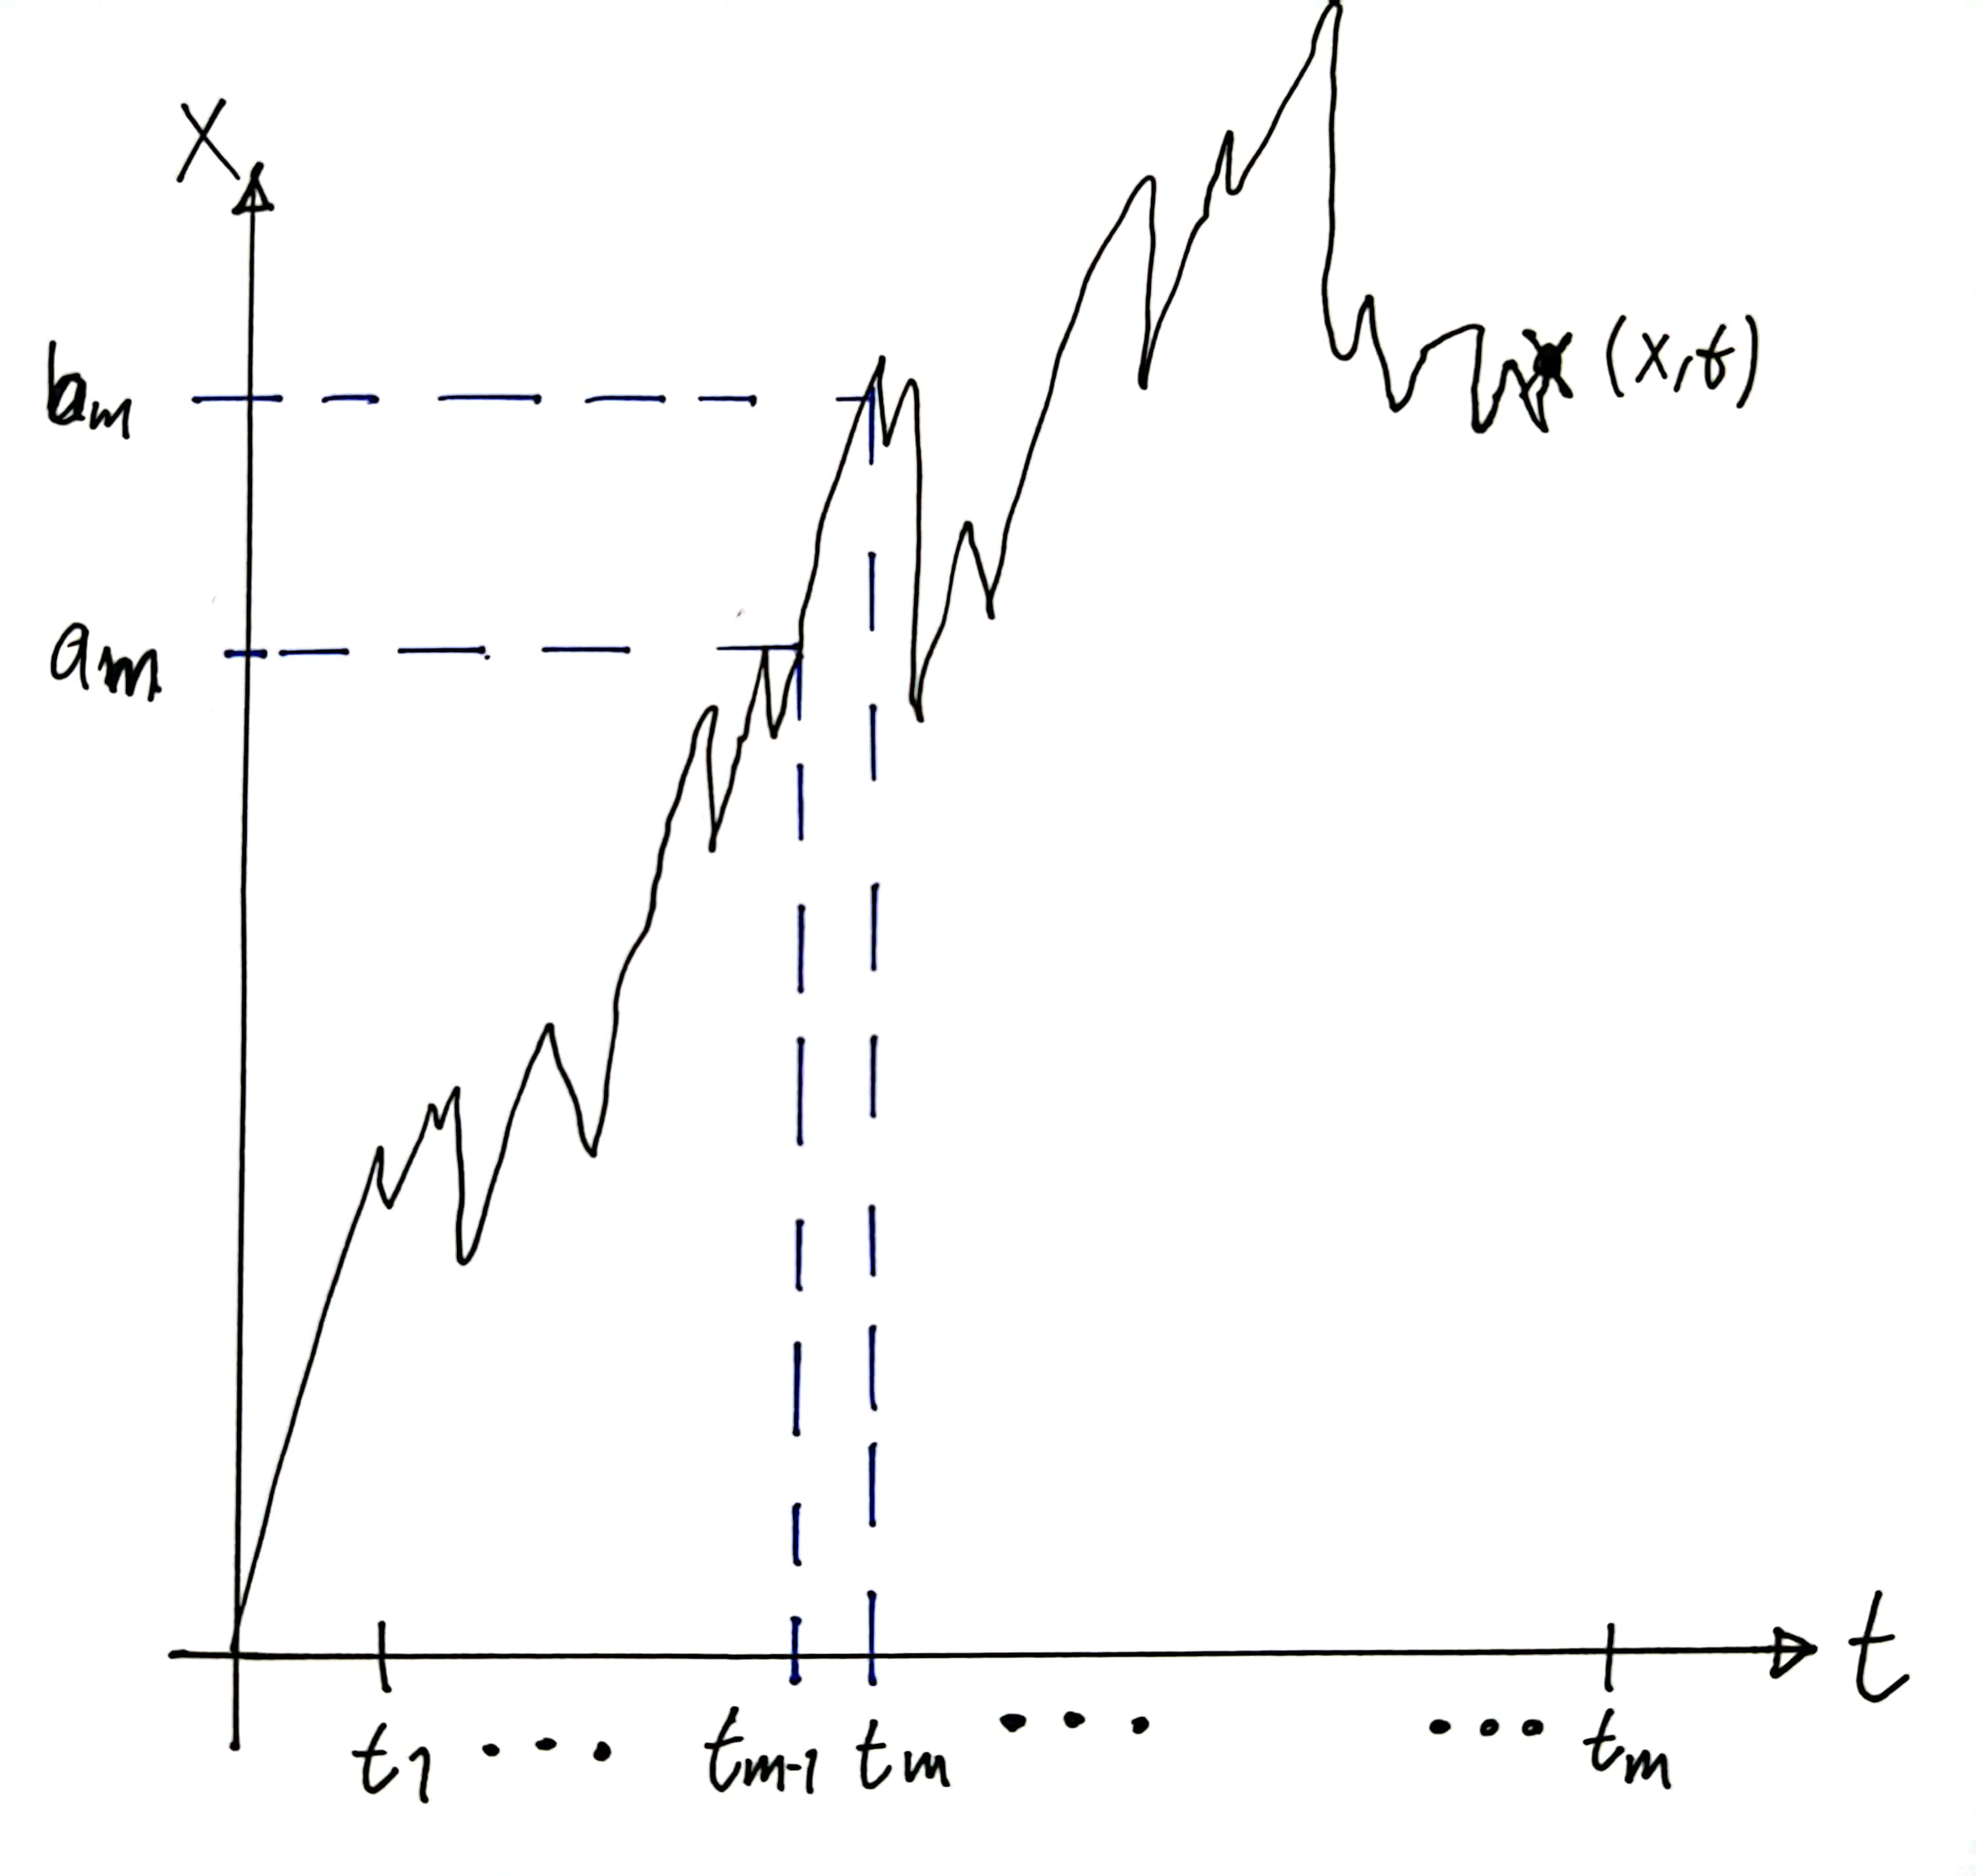
\includegraphics[width=.3\textwidth]{fig/path.jpg}
    \caption{A discretized path}
    \label{fig: path}
\end{figure}

As discussed around \autoref{eq: probability density}, when dealing with continuous space, and thus probability densities, the probability of finding a particle in the interval $(a, b)$ is
%
\begin{align}
    P(x\in (a, b), t ) = \int_a^b \dd x \, \Pe(\bm x, t).
\end{align}
%
To define probability density (``measure'') on an entier \emph{path}, and not just at isolated points, we discretize the path as
%
\begin{align}
    t_i &= i \Delta t, & i &\in [1, N], & t_N &= t, & x_i = x(t_i)
\end{align}
%
We consider paths with fixed endpoints, $x_0 = 0$, and $x_N = x$, as illustrated in \autoref{fig: path}.
A discretized path thus consists of finding the particle in certain intervals $(a_i, b_i)$ at times $t_i, i\in[1, N]$.
We define the probability measure of such a discretized path as
%
\begin{align}
    \Pe(x, t | x_i\in(a_i, b_i),\,  i \in 1, \cdots N )
    =
    \int\limits_{a_1}^{b_1} \dd x_1
    \cdots
    \int\limits_{a_{N-1}}^{b_{N-1}} \dd x_{N-1}\,
    \Pe(x, t | x_{N-1}, t_{N-1}) \cdots \Pe(x_{2}, t_{2} | x_{1}, t_{1}) \Pe(x_{1}, t_{1}) 
\end{align}
%
\todo[inline]{in the notes, the last integral is over $x_N$, but I assume it is $x_{N-1}$?}
Then, in the continuum limit, this becomes Brownian integral,
%
\begin{align}
    \D x(t)
    \equiv
    \lim_{\substack{|a_i-b_i|\rightarrow 0\\N \rightarrow \infty \\ t = \const}}
    \Pe(x, t | x_i\in(a_i, b_i),\,  i \in 1, \cdots N ).
\end{align}
%
This is a more careful definition of the path-integral measure defined in \autoref{section: introducing pi}.
In fact, this is a bone fide probability measure, as it has
%
\begin{enumerate}
    \item a \emph{sample space} (all paths)
    \item a $\sigma$-albebra \todo{define?}
    \item a measure on the sample space.
\end{enumerate}
%

\subsection*{Brownian functional}

Suppose $Q[x]$ is some \emph{functional} of the paths $x(t)$ with the form
%
\begin{align}
    Q[x] = \exp \left\{ - \int_0^t \dd \tau \, U(x(\tau)) \right\}.
\end{align}
%
We have already encountered such a functional in the Onsager-Machlup functional.
This is called a \emph{Brownian functional}.
In discretized form, this is a function $Q(x_1, \cdots x_{N-1})$.
Then, the expectation of this functional is\todo{Should we use $\E{\cdot } $ instead to be consistent?}
%
\begin{align}
    \mathbb{E}_{(x, t)}[Q]
    &
    \equiv
    \lim_{\substack{|a_i-b_i|\rightarrow 0\\N \rightarrow \infty \\ t = \const}}
    \int\limits_{a_1}^{b_1} \dd x_1
    \cdots
    \int\limits_{a_{N-1}}^{b_{N-1}} \dd x_{N-1}\,
    \Pe(x, t | x_{N-1}, t_{N-1}) \cdots \Pe(x_{2}, t_{2} | x_{1}, t_{1}) \Pe(x_{1}, t_{1}) 
    Q(x_1, \cdots x_{N-1}) \\
    &= \int\limits_{x(0) = 0}^{x(t) = x} \D x(t) \, Q[x].
\end{align}
%
We see immediately that $ \mathbb{E}_{(x, t)}[1] = 1$.
